\chapter{動作検証}
\thispagestyle{myheadings}
本研究の動作検証は特定の時空間に進入時のみセンシングできているか,プラットフォームとして複数のユースケースを想定して適切にセンシングできているかの2つを行う.

\section{時空間フェンシングの動作検証}
% 目的,環境,結果,考察
ジオフェンスが任意の多角形の時,マージンを含め適切に動作しているか検証した.
拡大したジオフェンスに進入した時に通知を発行し,縮小したジオフェンスに進入した時にセンシングが始まり,拡大したジオフェンスから退出した時にセンシングが終了していれば適切に動作しているとする.
動作検証の設定は図\ref{fig:ex_margin_1}に示す.

\begin{figure}[tbh]
    \centering
    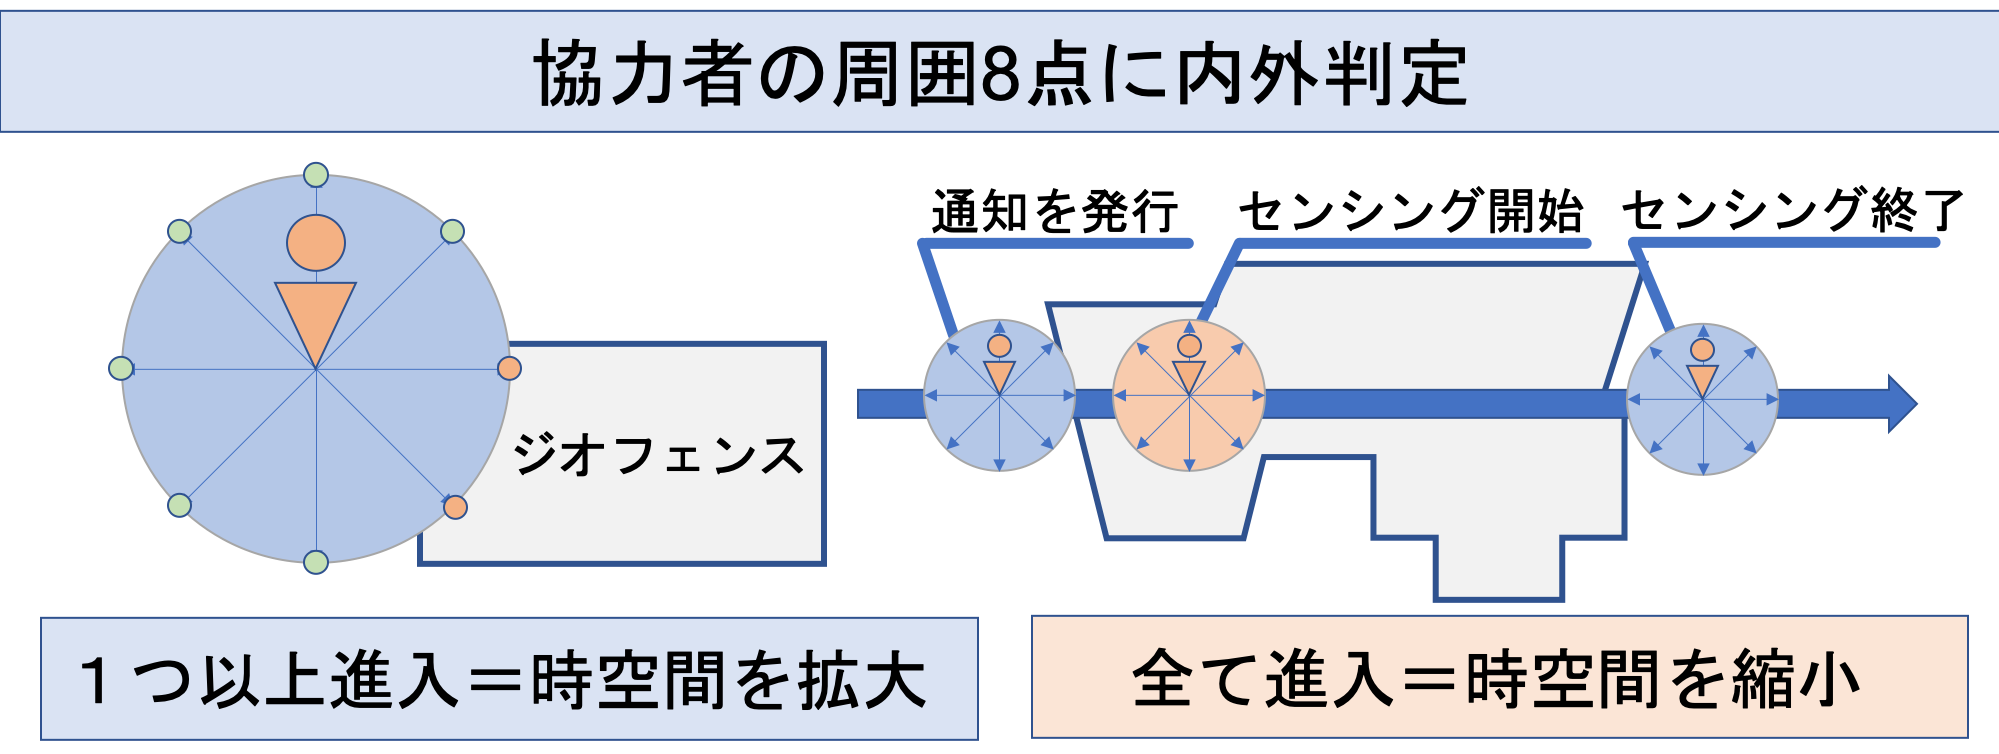
\includegraphics[width=16cm]{img_margin_2.png}
    \caption{時空間を拡大縮小するマージン}
    \label{fig:ex_margin_1}
\end{figure}

結果適切な動作が確認できた.
% (屋内でもやる)

\section{ユースケースを想定した動作検証}
まず,天候によって所要時間が変化する地図アプリを作成したい人がいたと仮定する.
時空間を歩行者の多い8時30分から16時50分の愛知工業大学と設定し,使用するセンサを線形加速度とGPSとした(図\ref{fig:ex_case_1}).

\begin{figure}[tbh]
    \centering
    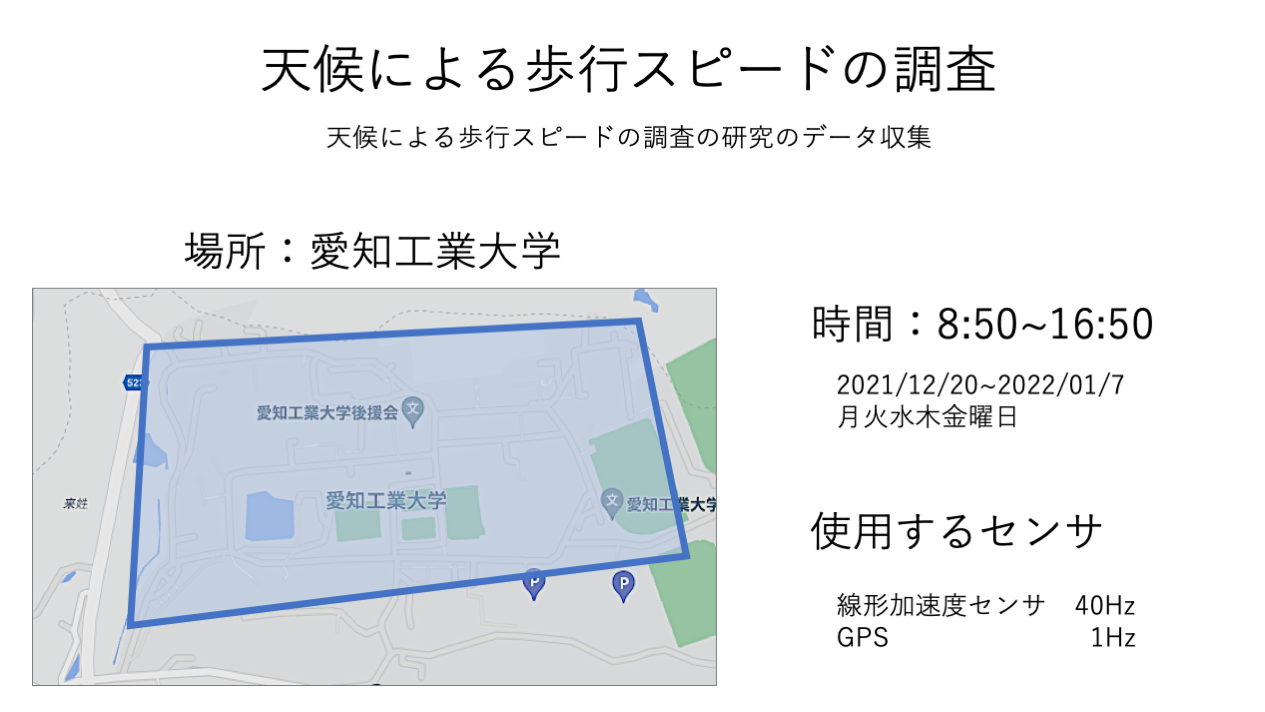
\includegraphics[width=16cm]{img_ex_case_1.png}
    \caption{天候によって所要時間が変化する地図アプリのためのクラウドセンシング}
    \label{fig:ex_case_1}
\end{figure}

結果,集めたセンサデータから移動速度と歩幅推定などができた.

次に,研究室の管理者が,研究室内でどれだけコミュニケーションが取られているか測定しようとしたと仮定する.
時空間を滞在者の多い8時30分から16時50分の研究室と設定し,使用するセンサを音センサとした.

\begin{figure}[tbh]
    \centering
    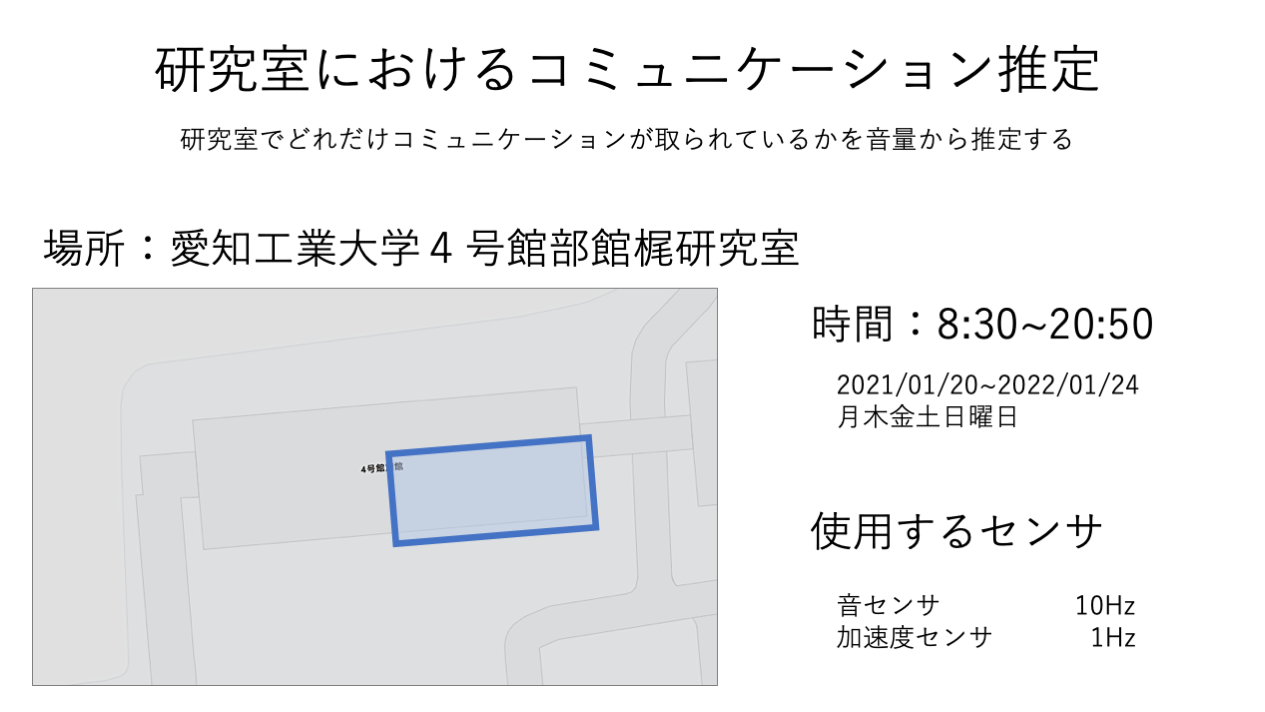
\includegraphics[width=16cm]{img_ex_case_2.png}
    \caption{天候によって所要時間が変化する地図アプリのためのクラウドセンシング}
    \label{fig:ex_case_2}
\end{figure}

結果,集めたセンサデータから時間帯ごとの賑やかさが推定できた.

% Local Variables: 
% mode: japanese-LaTeX
% TeX-master: "root"
% End: 
